%%%%%%%%%%%%%%%%%%%%%%%%%%%%%%%%%%%%%%%%%%%%%%%%%%%%%%%%%%%%%%%%%%%%%%
% How to use writeLaTeX: 
%
% You edit the source code here on the left, and the preview on the
% right shows you the result within a few seconds.
%
% Bookmark this page and share the URL with your co-authors. They can
% edit at the same time!
%
% You can upload figures, bibliographies, custom classes and
% styles using the files menu.
%
%%%%%%%%%%%%%%%%%%%%%%%%%%%%%%%%%%%%%%%%%%%%%%%%%%%%%%%%%%%%%%%%%%%%%%

\documentclass[12pt]{article}
\usepackage{float} 
\usepackage[utf8]{inputenc}  
\usepackage[inline]{enumitem}

\usepackage{sbc-template}
\usepackage{tabularx}
\usepackage{float}
\usepackage{graphicx,url}
\usepackage{graphicx}
\usepackage{microtype}

\usepackage[brazil]{babel}   
\usepackage{tcolorbox}
\usepackage[inline]{enumitem}

\sloppy

\title{Benefícios da Aplicação da Etapa de Medição do \textit{Lean Learning}: um estudo de
caso no ensino da Engenharia de \textit{Software}}

\author{Davi B. Saldanha\inst{1}, Gabriel S. Barroso\inst{1}}


\address{Instituto de Ciências Exatas e Informática\\ Pontifícia Universidade Católica de Minas Gerais
  (PUC - MG)\\
  Belo Horizonte -- MG -- Brasil
  \email{davi.brandao@sga.pucminas.br, gsbarroso@sga.pucminas.br}
}

\begin{document} 

\maketitle

\begin{abstract}
  Lean Learning is a methodology that aims the constant improvement of learning processes, in order to increase quality and productivity of teachers and students. As its name indicates, it is an adaptation of the Japanese management model named Lean Management, which is applicable to many industry sectors. The study of the application of Lean principles in education is still recent, but promising on promoting better adequacy between public and content. This article analyzed one step that is part of the Lean Learning cycle, named Measure, applied to the context of Software Engineering teaching. An exploratory study case was made, based on application of quizzes to students and teachers, to collect their opinion about the application of practical exercises. The results were positive and showed that the use of the methodology can be beneficial to the Software Engineering course.
  
  \textbf{Keywords:} \emph{Lean, Lean Learning, Software Engineering}
\end{abstract}
     
\begin{resumo} 
  Lean Learning é uma metodologia que visa a melhoria constante dos processos de aprendizagem, buscando aumentar qualidade e produtividade para professores e alunos. Como seu nome indica, ela se trata de uma adaptação do modelo japonês de gestão denominado Lean Management, aplicável a diversos setores de indústria. O estudo da aplicação dos princípios Lean na educação é recente, mas promissor no sentido de promover melhor adequação entre público e conteúdo. Este trabalho analisou uma das etapas previstas no ciclo do Lean Learning, denominada Medir, aplicada ao contexto do ensino da Engenharia de Software. Para tal, fez-se um estudo de caso exploratório, por meio da aplicação de questionários a alunos e professores, observando sua opinião sobre a aplicação de práticas. Os resultados foram positivos e indicaram que o uso da metodologia pode ser benéfico para o curso de Engenharia de Software. 
    
  \textbf{Palavras chave:} \emph{\textit{Lean}, \textit{Lean Learning}, Engenharia de \textit{Software}}
\end{resumo}

\begin{tcolorbox}
\footnotesize
\textbf{Bacharelado em Engenharia de \emph{Software} - PUC Minas\\
Trabalho de Conclusão de Curso (TCC)} \\

\indent Orientador de conteúdo (TCC I): José Laerte Pires Xavier Junior - laertexavier@gmail.com\\
Orientador acadêmico (TCC I): Lesandro Ponciano dos Santos - lesandrop@pucminas.br\\
Orientadora do TCC II: Letícia Castro Peixoto - leticiacastropeixoto@pucminas.br\\ \\
Belo Horizonte, 14 de maio de 2021.
\end{tcolorbox}

\newpage

\section{Introdução}

A área de desenvolvimento de \textit{software} atualmente conta, em grande parte, com metodologias de desenvolvimento ágil e práticas derivadas dos princípios do \textit{Lean Management} \cite{poth2019lean}. Oriundo do Japão, o \textit{Lean} consiste numa filosofia de gestão criada a partir do modelo toyotista de produção, que busca eliminar ao máximo os desperdícios dos recursos envolvidos na cadeia produtiva, resolver problemas sistematicamente e mudar a forma de visualizar e gerenciar um negócio \cite{shingo2019study}. Por se tratar de um modelo orientado a processos, métricas e conceitos, o \textit{Lean} é amplamente aplicável a empresas de diversos setores.

Estudos recentes apontam a dificuldade em lecionar com qualidade o conteúdo relacionado à Engenharia de \textit{Software}, devido a quantidade de informações e relevância da área \cite{EnsinoEng2014} \cite{chatley2017lean} \cite{marques2017enhancing}. Com o objetivo de transmitir o máximo de conteúdo da área, costuma-se realizar atividades práticas com os alunos \cite{EnsinoEng2014}. O livro de Chatley, ``Agile and Lean Concepts for Teaching and Learning" \nocite{ChatleyBook2019}, traz maneiras de se aplicar o \textit{Lean Learning} no ensino da Engenharia de \textit{Software}. Também mostra dois caminhos a serem seguidos quando se utiliza o \textit{Lean Learning}. O caminho tradicional visa modificar o ensino comum buscando \textit{feedback} constante e o caminho orientado a projetos busca ensinar por meio da prática simulada de determinada teoria.

O principal problema que este trabalho analisa é a ausência de medidas da eficácia de ferramentas \textit{Lean} no ensino da Engenharia de \textit{Software}. Para tanto, o estudo avalia a aplicação de práticas em sala de aula e explora aspectos do nível de satisfação, adequação e proximidade com o mercado de trabalho, buscando assim aproximar o aprendizado aos conceitos ágeis do \textit{Lean}. Em função deste problema, este trabalho se propõe a investigar a implementação da etapa \textit{Measure} (Medir) do \textit{Lean Learning} e seu potencial de trazer melhoria contínua para o aprendizado da Engenharia de \textit{Software}. A escolha dessa etapa se dá pelo fato de ser nela que ocorre a coleta de informação, a fim de receber \textit{feedback} qualitativo dos alunos. É a partir desse retorno que se pode buscar melhorias no ensino, fazendo desta etapa a mais importante para o processo.

O objetivo geral deste trabalho é avaliar empiricamente a aplicação da fase de medição da metodologia \textit{Lean Learning} no ensino da Engenharia de \textit{Software}, a fim de potencializar a produtividade e qualidade do ensino. Também existem objetivos específicos, estes sendo: i) propor uma abordagem de aplicação da etapa \textit{Measure} do \textit{Lean Learning} em disciplinas de Engenharia de \textit{Software}; ii) avaliar a aplicabilidade da metodologia no contexto da Engenharia de \textit{Software}; iii) obter a percepção de professores e alunos acerca da abordagem proposta.

O trabalho se divide em seis seções. A Seção 2 apresenta mais conceitos importantes e detalhes sobre as abordagens de implementações da metodologia \textit{Lean Learning}. A Seção 3 descreve os principais trabalhos relacionados. A Seção 4 detalha e discute a metodologia aplicada no experimento. Na Seção 5 ocorre a análise estatística dos resultados obtidos. Na Seção 6 encontram-se a conclusão e as considerações finais deste trabalho.

\section{Referencial Teórico}

Esta seção do trabalho apresenta termos e conceitos de importância para a realização do experimento. O trabalho abrange conceitos sobre as metodologias ágeis de desenvolvimento e sobre o modelo toyotista de produção com o nome de \textit{Lean}.

\subsection{Métodos ágeis}

Desenvolvimento ágil é o termo utilizado para representar um conjunto de métodos e práticas adotados para desenvolver e entregar \textit{software} de forma rápida e incremental. As metodologias ágeis são derivadas dos valores e princípios contidos no Manifesto Ágil \cite{Manifesto}. As metodologias de desenvolvimento que surgiram a partir do Manifesto são diversas, sendo as mais populares \textit{Scrum e Extreme Programming} (XP) \cite{poth2019lean}. Nas metodologias de desenvolvimento ágil, pode-se observar semelhanças como a organização em equipes pequenas, menor hierarquização e burocratização, ciclos curtos, iterativos e incrementais de entrega e o foco na geração rápida de valor \cite{wei2019}. Com base nos fatores de sucesso observados na utilização de métodos ágeis pela indústria, acredita-se que seu uso no ensino acadêmico também possa ser bem sucedido \cite{fernandes2019identifying}.

\subsection{Metodologia \textit{Lean} e derivados}

O processo do \textit{Lean Learning} -- que será explicado mais a frente nesta seção --, possui três fases, sendo denominadas \textit{``Build, Measure e Learn"} ou ``Construir, Medir e Aprender", representadas pelos círculos azuis na Figura 1. Já os círculos verdes representam os artefatos gerados após cada fase. Após a etapa de aprender, ideias de como melhorar o ensino surgem. Depois da fase de construir, geram-se protótipos de atividades práticas para fixar o conteúdo lecionado. Após a fase de medir, dados aparecem em forma de métricas a serem avaliadas e, após essa avaliação, repete-se o ciclo em busca da melhoria contínua do aprendizado. Novamente é necessário aprender como melhorar o ensino, construir novas formas de lecionar e medir os resultados obtidos no ciclo.

\begin{figure}[!h]
    \centering
    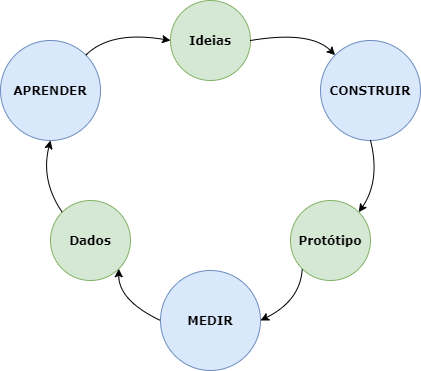
\includegraphics[width=7cm,height=5.9cm]{Imagens/Lean.png}
    \caption{Processo \textit{Lean Learning}. Fonte: autores}
    \label{fig:Processo}
\end{figure}

O \textit{Lean} visa a constante otimização dos processos produtivos e a qualidade do produto entregue. Os frutos desse modo de pensar promovem menor desperdício de recursos, redução de custos, aumento de velocidade de produção e geração de valor para o cliente. Além desses benefícios para o negócio, ele também acarreta numa harmonização maior para a equipe que, com melhores resultados, fica mais satisfeita com seu trabalho \cite{poth2019lean}.

O \textit{Lean} possui três palavras (em japonês) essenciais sobre os seus valores, sendo elas: (i) \textit{Mura}, (ii) \textit{Muri} e (iii) \textit{Muda}. \textit{Mura} significa evitar qualquer processo ou prática que não seja estável. \textit{Muri} significa evitar tarefas que possam sobrecarregar processos, pessoas e equipamentos. E \textit{Muda} significa eliminar atividades e processos identificados como inúteis e que estejam dificultando o gargalo das atividades.

O \textit{Lean Learning} consiste no uso do \textit{Lean} voltado à educação. Assim como na forma de ensino comum nas escolas e universidades, o \textit{Lean Learning} possui seus papéis \cite{chatley2017lean}. Há o papel do professor, conhecido como especialista, há o estudante e, por último, há o papel de líder. O especialista é quem leciona as disciplinas propostas e auxilia os alunos a entender o conteúdo. Os estudantes, por sua vez, serão os aprendizes do professor e realizam tarefas propostas e são avaliados pelo desempenho obtido nas atividades. O líder pode ser a mesma pessoa do professor -- seu papel é assegurar suporte institucional para o método ser devidamente aplicado. Além disso, ele incentiva uma presença mais ativa dos professores e dos demais funcionários do ambiente \cite{madruga2018}.

O processo se inicia na fase de aprender, onde é definido o que se quer aprender. Na abordagem de Boufleur et al. (2016) sobre o \textit{Lean Learning}, busca-se descobrir práticas redundantes e que não estão diretamente ligadas ao ensino. Anotação da teoria do conteúdo, inicialização a um novo tema na disciplina, atividades como estas não são focadas propriamente no aprendizado dos alunos sobre determinado assunto, mas no registro deste. Nessa fase geram-se ideias, que seriam o artefato de um cronograma de aulas, onde o professor define o que ele irá lecionar ao longo do período, quando as atividades práticas e provas irão ocorrer, quando revisar matérias entre outras atividades.

Após a fase de aprender, deve-se realizar a fase de construir, na qual é feito um novo projeto educacional visando a maior satisfação dos alunos. Como o \textit{Lean Learning} foca em atividades práticas para se fixar o conteúdo da disciplina com os alunos, nessa fase de construir geram-se os protótipos. Essas são as ideias das atividades práticas aplicadas aos alunos. Define-se o porque essa prática pode ser útil aos alunos e a qual parte da matéria lecionada ela se relaciona \cite{LeanStartup2016}. Um exemplo comum na Engenharia de \textit{Software} é a prática de montagem de aviões de papel, simulando uma rotina de trabalho em equipe com a metodologia \textit{Scrum} em uma empresa.

Por último, na fase de medir, são analisados os \textit{feedbacks} dados pelos estudantes e aplica-se o que achar necessário em busca de melhorias no ensino, seja em questão de gastos, tempo ou no desempenho dos alunos. Ao medir determinadas métricas de eficiência, dados são gerados. Esses dados informam ao professor se determinada prática foi útil ou não aos alunos, e permite ao professor retornar à fase de aprender sabendo qual atividade prática deve ser reaproveitada em outro período, e qual seria necessário ser reformulada para se tirar maior proveito dela. A etapa de medir utiliza das atividades práticas para gerar os dados que são analisados e servem como \textit{feedback} para o professor.

O \textit{Lean Learning} é um processo repetitivo, onde em cada ciclo se busca uma melhoria contínua, como visto na Figura 1. Portanto, ao acabar a fase de construir, é necessário novamente buscar possíveis novos gargalos ou atividades negativas no novo método educacional, a fim de otimizá-lo novamente \cite{LeanStartup2016}. Alguns dos artefatos produzidos ao se utilizar o processo do \textit{Lean Learning} são: ementa da disciplina, escopo de atividades práticas, provas, cronograma de aulas, trabalhos realizados, apresentações gravadas e artigos escritos.

\section{Trabalhos Relacionados}

Os artigos relacionados a este trabalho estão ligados a métodos e satisfação do ensino em geral e especializado na engenharia de \textit{software}, desenvolvimento ágil e na metodologia \textit{Lean}. Como este trabalho busca analisar a aplicação de um modelo \textit{Lean} para o ensino, são citados inicialmente artigos que abordam como ensinar de maneira efetiva e satisfatória.

%No artigo de Nowostawski et al. (2018)\nocite{gamifying2018}, é abordado um método de ensino que tem crescido ultimamente, a  \textit{Gamification}. Para este trabalho, há um maior proveito da sessão que aborda a satistação dos aprendizes. O artigo quer demonstrar como a gamificação pode apresentar melhoras no ensino da engenharia de \textit{software}, tanto em qualidade quanto em interesse dos alunos. Para isso, eles criaram uma metodologia de ensino à parte, chamada \textit{The Game of Reading and Discussion}. Durante 4 anos (2015-2018) essa metodologia foi aplicada e consistia basicamente em fazer os alunos lerem artigos, elaborarem perguntas sobre os artigos e após isso, realizar uma reflexão dos artigos lidos e avaliar a reflexão de algum outro aluno. E ao final os números mostram que os alunos estão mais engajados nas aulas.

%\nocite{marques2017enhancing}Marques et al. (2017) citam sobre os métodos ágeis no ensino do desenvolvimento de \textit{software}. Grande parte das instituições de ensino começam a lecionar o desenvolvimento de \textit{software} de maneira extremamente focada no desenvolvimento ágil. Porém nem sempre essa pode ser a maneira mais adequada de se ensinar a construir \textit{softwares} para programadores novatos. O método de reflexão semanal de desempenho (RWM, ou Reflexive Weekly Monitoring) é abordado no artigo, alegando que este método de início seria mais efetivo e coordenado, além de os alunos se sentirem mais satisfeitos e prestativos com a sua equipe. O RWM busca principalmente desenvolver as competências dos alunos, como a vontade de aprender, adaptação a ferramentas entre outras. Como o artigo trata de uma conexão entre metodologias ágeis -- que são técnicas utilizadas pelo mercado -- e aprendizagem, seu tema conecta-se ao deste trabalho, na medida em que analisa a combinação entre métodos ágeis e uma metodologia para avaliação de desempenho na aprendizagem.
\nocite{EnsinoEng2014}Santos et al. (2014) abordam em seu artigo métodos e experimentos de ensino na engenharia de \textit{software} como disciplina da área de informática. O artigo sempre aborda o fato do amplo conteúdo que a engenharia de \textit{software} abrange e sua importância para a qualidade dos sistemas gerados. Devido a grande quantidade de conteúdo, se tornou necessário a utilização de métodos diferentes de ensino na tentativa de repassar a base da engenharia de \textit{software} de forma adequada. Para atingir o objetivo do artigo, a principal abordagem utilizada pelos autores, foi a aplicação de atividades práticas na disciplina, método que se assemelha a um dos princípios do \textit{Lean Learning}.

\nocite{chatley2017lean}Chatley e Field (2017) abordam como aprende-se algo, reforçando a ideia de práticas durante o aprendizado, em vez de apenas materiais de pesquisa e textos repetitivos dos livros escolares. Segundo a metodologia \textit{Lean}, é possível evitar o desperdício de recursos materiais e de tempo caso o ensino seja conduzido da maneira correta. Como eles utilizaram o \textit{Lean} no ensino, prezaram fortemente por um \textit{feedback} rápido e ciclos iterativos curtos, para assim manter o contato com os 150 alunos da Universidade Imperial. Decidiram utilizar essa abordagem ágil para familiarizar os alunos com o mercado atual. Também defendem que o ensinamento real vem da prática, sendo o ensino teórico apenas a base. A abordagem é positiva, visto que incentivam o uso de técnicas do mercado que se demonstraram bem sucedidas, como a programação em pares e ideias semelhantes a \textit{Hackathons}. Como este trabalho aplica uma análise sobre as práticas realizadas em disciplinas em conjunto com o \textit{Lean Learning}, o artigo de Chatley e Field é uma referência fundamental.

%Metodologias ágeis
Dentre os artigos que abordam as metodologias ágeis e \textit{Lean},\nocite{poth2019lean} Poth et al. (2019) apresentam a eficiência e a melhora produtiva ao se utilizar o \textit{Lean} e metodologias ágeis em conjunto. Seu artigo busca analisar as abordagens \textit{Lean} e \textit{Agile SPI (Software Process Improvement)} em ambientes de desenvolvimento tradicionais e ágeis e demonstrar que em ambos os cenários é possível buscar essas abordagens. São pontuados os princípios chave do \textit{Lean Software Development} e então revisitam o Manifesto Ágil. Essa construção permite ao leitor perceber as conexões existentes desde o surgimento do \textit{Lean} e seus processos de qualidade e melhoria e seus princípios. Então, há uma análise de SPI em ambientes tradicionais e ágeis e são discutidas as abordagens para cada um. Como este trabalho visa analisar as consequências da aplicação dessas metodologias em uma graduação em Engenharia de \textit{Software}, o trabalho de Poth et al. (2019) serve como referência a esta pesquisa.

%\nocite{fernandes2019identifying}Fernandes e Barcelos (2019), em sua pesquisa sobre a aplicação de metodologias ágeis a projetos de reengenharia de \textit{software}, fazem menção aos resultados observados por outros trabalhos. Estes, mostram que os métodos ágeis mais utilizados na indústria brasileira de \textit{software} são \textit{Scrum} e XP, e os benefícios de seu uso. Os resultados do projeto foram comparados com a percepção do time de desenvolvimento por meio de entrevistas semiestruturadas, com a análise dos artefatos do projeto e as melhores práticas propostas na literatura para entender se os resultados mencionados nesta última seriam confirmados pela prática. Os resultados da pesquisa de Fernandes e Barcelos indicam que o produto da reengenharia foi bem sucedido, de acordo com os \textit{stakeholders} do projeto. A utilização de metodologias ágeis foi reconhecida como fator de sucesso.

%O trabalho de Miranda et al. (2019)\nocite{wei2019}, que estuda o impacto do \textit{Scrum} no sucesso de projetos de \textit{software}, sinaliza sobre a aplicação de metodologias ágeis no meio acadêmico. Nas considerações finais do artigo, destaca-se o engajamento dos alunos que participaram do estudo, em relação ao \textit{Scrum} e seus benefícios. Apesar de exigir maior dedicação para se aprender a metodologia nova, o resultado observado foi positivo.

%A decisão de criar questionários e realizar entrevistas para obter os resultados do trabalho partiu de dois trabalhos, sendo eles o de Bandeira (2003)\nocite{Questionarios1} e de Henkel (2017)\nocite{Questionarios2}. Em ambos são apresentados métodos para análise de respostas abertas e fechadas em questionários. Para os resultados deste trabalho, utiliza-se parte dos métodos descritos por ambos, onde é necessário interpretar a fundo as respostas abertas e explorar as métricas obtidas com as respostas fechadas.

\section{Metodologia}

%Tipo de pesquisa e sua justificativa
Este trabalho se trata de um estudo de caso, pois se avalia o \textit{Lean Learning} em um contexto da vida real, com finalidade de pesquisa empírica, visando aprofundar os estudos na área \cite{MIGUEL2007}. Além disso, não há aprioristicamente um esquema estrutural, não tendo um problema e variáveis já definidas previamente, portanto seu objetivo é apreender determinada situação e descrever o caso observado\cite{marconi2003fundamentos}\cite{marconi2012tecnicas}. Também é descritivo, já que apresenta uma descrição exaustiva de um fenômeno, dentro do respectivo contexto \cite{Eduser} a fim de refinar os estudos sobre a teoria \cite{MIGUEL2007}. Envolve medidas qualitativas como a satisfação dos alunos e do professor com as atividades propostas com o \textit{Lean Learning} e gera métricas quantitativas para análise geral dos resultados obtidos, como a média da satisfação geral dos alunos quanto às atividades realizadas \cite{Metricas}. Como objeto de estudo do trabalho tem-se a etapa \textit{Measure} (Medir) do \textit{Lean Learning}.

Com os dados coletados, é conduzida a fase de análise dos mesmos. Procura-se observar possíveis padrões presentes nas métricas abordadas no trabalho, e descrever situações que foram benéficas para a satisfação dos alunos. A cada questionário fechado analisado, é definida a média das métricas coletadas em relação a todos os alunos respondentes. Além disso, através de um \textit{script} R, será possível estabelecer quais perguntas possuem correlação com as métricas estudadas, através do uso da função \textit{cfa()} (de Análise Fatorial Confirmatória), da biblioteca lavaan (\textit{latent variable analysis}). 

As nove perguntas relativas às práticas presentes no questionário fechado dos alunos foram agrupadas em três tipos: três perguntas para medir satisfação (S), três perguntas para medir adequação (A) e três perguntas para medir a proximidade da prática com o mercado (M). O primeiro grupo visa avaliar a satisfação dos alunos com a realização da prática. O segundo visa avaliar a opinião dos alunos sobre sua adequação à prática, em termos de cumprimento, dificuldade e tempo disponível. O terceiro e último visa avaliar a opinião dos alunos sobre o quanto a prática reflete a realidade do mercado de trabalho de \textit{software}.

A fórmula para a especificação de modelos de regressão no Lavaan se da pela seguinte notação:

$y_{i} = \beta_{0} + \beta_{1}x_{1i} + \beta_{2}x_{2i} + \beta_{3}x_{3i} + \epsilon_{1}$

Onde $\beta_{0}$ é o intercepto, os betas de 1 a 3 são os coeficientes de regressão para cada uma das variáveis do modelo desse trabalho e $\epsilon_{i}$ é o erro residual para a observação ``i". Passando o modelo para o ambiente R, temos a seguinte notação:

$S =\sim X_{1} + X_{2} + X_{3}$

$A =\sim X_{4} + X_{5} + X_{6}$

$M =\sim X_{7} + X_{8} + X_{9}$

Onde, no modelo dessa pesquisa, S representa o nível de satisfação dos alunos, A o nível de adequação da prática e M a proximidade da prática com o mercado. Estas são as variáveis latentes dependentes do trabalho. $X_{1}$ a $X_{9}$ representam as valores obtidos através das perguntas realizadas no questionário dos alunos, essas representam as variáveis independentes . O sinal de til ($\sim$) representa para o R uma operação de regressão, ao utilizar esse sinal, o ambiente R já estima o valor do intercepto e do erro residual, portanto não é necessário explicitá-los na construção do modelo.

A função \textit{cfa()} do pacote lavaan é uma função específica para a análise de modelos fatoriais confirmatórios, o primeiro objeto da função é o que contém a sintaxe do modelo, o segundo representa o conjunto de dados a ser observado. Essa função define automaticamente a variância e covariância das variáveis observadas e latentes, os resultados obtidos serão discutidos na seção 5.


$info \leftarrow `` S =\sim X_{1} + X_{2} + X_{3}$

$A =\sim X_{4} + X_{5} + X_{6}$

$M =\sim X_{7} + X_{8} + X_{9} " $

$fit \leftarrow cfa(info,\ data = dtF)$

\subsection{Etapas}
Nesta subseção são apresentadas quais são as etapas previstas nos cronogramas:

    \begin{enumerate}\setlength\itemsep{0.5em}
        %\item Entrar em contato com professores dispostos a ajudar no experimento.
        %\item Desenvolvimento do questionário fechado destinado aos alunos para medir sua satisfação com o %aprendizado.
        %\item Desenvolvimento do questionário fechado destinado aos professores para medir sua percepção do %progresso dos alunos.
        %\item Desenvolvimento do questionário aberto destinado aos alunos para obter suas considerações %quanto ao processo de aprendizagem.
        %\item Elaboração de uma entrevista semiestruturada aos professores para obter suas considerações %sobre o andamento das disciplinas e o processo descrito.
        \item Apresentação do experimento nas disciplinas.
        \item Aplicação da atividade prática 1.
        \item Aplicação da atividade prática 2.
        \item Aplicação da atividade prática 3.
        \item Aplicação do questionário aberto aos alunos.
        \item Aplicação do questionário fechado aos alunos.
        \item Aplicação do questionário fechado aos professores.
        \item Análise dos resultados obtidos na aplicação dos questionários.
        \item Escrita e revisão do documento final.
    \end{enumerate}

\subsection{Procedimentos}

\begin{figure}
    \centering
    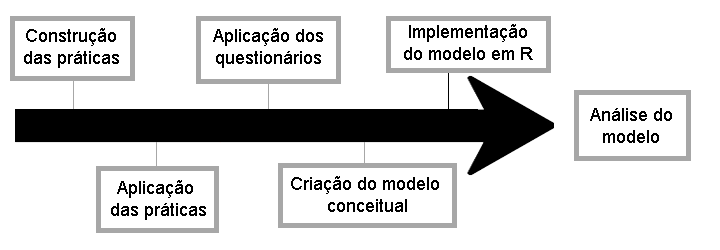
\includegraphics[width=14cm,height=4cm]{Imagens/Procedimento.png}
    \caption{Procedimentos}
    \label{fig:Procedimento}
\end{figure}

Nesta subseção encontram-se as descrições dos artefatos a serem utilizados no experimento e das etapas a serem cumpridas. A realização do experimento ocorre por meio da aplicação de questionários (online via \textit{Google Forms}) -- cujos detalhes são debatidos a seguir --, a fim de colher \textit{feedbacks} sobre a satisfação dos alunos com o processo de aprendizagem e sobre a percepção do professor do desempenho da turma \cite{chatley2017lean}. As perguntas são focadas em medir o quanto as atividades práticas nas disciplinas sobre as quais o experimento é executado estão agregando à formação dos alunos, em termos de fixação de conhecimento e conformidade com as demandas do mercado de trabalho \cite{chatley2017lean}. Busca-se tentar compreender se existe a percepção de que determinadas atividades e conhecimentos não são úteis ou são menos relevantes em detrimento de outros.

A decisão de criar questionários para obter os resultados do trabalho partiu de dois trabalhos, sendo eles o de Bandeira (2003)\nocite{Questionarios1} e de Henkel (2017)\nocite{Questionarios2}. Em ambos são apresentados métodos para análise de respostas abertas e fechadas em questionários. Para os resultados deste trabalho, utiliza-se parte dos métodos descritos por ambos, onde é necessário interpretar a fundo as respostas abertas e explorar as métricas obtidas com as respostas fechadas.

%Para o experimento espera-se conseguir o auxílio de dois professores especialistas do curso da Engenharia de \textit{Software}, dispostos a ajudar na experimentação da metodologia \textit{Lean Learning} durante um período letivo em sua disciplina. Com isto, espera-se que aproximadamente sessenta alunos participem do experimento. A escolha do especialista foi baseada em: i) seu conhecimento prévio sobre \textit{Lean}; ii) relação da sua disciplina com a metodologia; iii) período que a disciplina está alocada no curso. Busca-se abranger alunos iniciados e experientes, possibilitando uma amostragem diversificada de alunos e especialistas.
Para o experimento, conta-se com o auxílio da professora -- conhecida como especialista, conforme os atores especificados pelo processo do \textit{Lean Learning} -- do curso de Engenharia de \textit{Software} da PUC Minas, que lecionará a disciplina de Gestão da Produção de \textit{Software} no primeiro semestre de 2021. Ela foi contatada pelos autores e concordou em ajudar na experimentação da metodologia durante um período letivo em sua disciplina. Como espera-se atingir uma massa de pelo menos 60 respostas, outros professores foram contatados para contribuição no experimento. A escolha do professor (especialista) é baseada em: i) relação da sua disciplina com metodologias ágeis, processos de software e gestão \textit{Lean} e ii) período em que a disciplina está alocada no curso. 

Como há a possibilidade de as disciplinas selecionadas para o trabalho sofrerem conflito (concorrência) de horários e pelo menos um dos dois pesquisadores deve acompanhar a execução das práticas em cada disciplina no decorrer do semestre, eles podem ter que se dividir na execução destas. Essa divisão compreende também a aplicação dos questionários.

Busca-se trabalhar com alunos que estejam matriculados em disciplinas do segundo período em diante, pois supõe-se que normalmente é a partir desse momento que estão começando a adentrar o mercado de trabalho (ou estão próximos disso). Essa suposição é feita com base nos conhecimentos adquiridos até o terceiro período, pois nesta fração do curso os alunos já aprenderam alguns conteúdos basilares da Engenharia de \textit{Software}, como Algoritmos e Estruturas de Dados e Programação Modular, por exemplo -- e com esses conhecimentos, já estão minimamente aptos a ingressar no mercado de trabalho, ocupando cargos de entrada. Também é suposto que esses alunos sejam capazes de analisar por conta própria os benefícios do aprendizado na academia em seu dia a dia profissional, visto que já trabalham na área.

\subsubsection{Descrição das atividades práticas}

Neste trabalho espera-se estudar a etapa de Medir. Para isso, foram propostas atividades práticas -- em conjunto com a professora de Gestão da Produção de \textit{Software} -- que serão acompanhadas pelos autores deste trabalho e servirão como os protótipos no desenho do processo. Essas atividades são: 

    \begin{enumerate}\setlength\itemsep{0.5em}
        \item Prática envolvendo compreensão e refinamento de requisitos de software.
        \item Prática envolvendo trabalho em equipe, velocidade e competitividade.
        \item Prática envolvendo trabalho em equipe, brainstorming, criatividade e comunicação.
    \end{enumerate}

Na prática 1 propõe-se que os alunos se organizem em trios. Um dos alunos deve elaborar requisitos para uma tela de um sistema de sua escolha. Apenas através de texto, os requisitos da tela devem ser descritos e passados para os outros dois alunos. Ao receberem os requisitos, os dois devem ilustrar uma tela (na ferramenta de sua escolha) de acordo com as especificações dadas, de forma individual. Ao final da elaboração das telas, haverá uma reflexão com os alunos mediada pelo professor, sobre o que se esperava na tela e porque a tela foi feita daquela maneira. Espera-se que seja possível analisar pontos da etapa da elicitação de requisitos, como a fragilidade de requisitos ambíguos ou mal descritos e também como a interpretação dos requisitos pode alterar o resultado. Estima-se que essa atividade prática demande 30 minutos.

Na prática 2 uma lista contendo 4 problemas de programação serão apresentados aos alunos, que devem se organizar em grupos de 3 ou 4 integrantes. Durante 30 minutos eles devem resolver o máximo de problemas que conseguirem, podendo se organizar como quiserem -- decidindo como será a divisão de tarefas entre os membros, quais linguagens, recursos e ferramentas serão utilizados etc. Essa prática possui quatro restrições: 
    \begin{enumerate}\setlength\itemsep{0.5em}
        \item Os alunos terão apenas 30 minutos para a resolução dos problemas;
        \item Todos os integrantes dos grupos devem atuar na resolução dos problemas (ou seja, nenhum deve ficar ocioso);
        \item Todos os grupos formados devem operar de forma individual, não podendo haver cooperação entre eles;
        \item Ao final do tempo dedicado à resolução dos problemas, os alunos devem entregar um arquivo compactado (.zip, .rar ou .tar) contendo todas as soluções, de modo a garantir que nenhum código se altere após o prazo.
    \end{enumerate}
Para avaliar a resolução dos problemas, serão verificados apenas os conjuntos de saídas para cada conjunto de entradas testado, desconsiderando a implementação adotada no código. Essa atividade visa estimular trabalho em equipe, agilidade, coordenação e uma competição saudável entre os alunos. De modo a estimular a competição, será negociada a possibilidade de dar pontos extras (até 2) como prêmio aos membros da equipe vencedora, em cada disciplina em que a prática for aplicada. Essa atividade prática demanda 30 minutos. Os problemas de programação encontram-se no apêndice deste trabalho. 

 Na prática 3, os alunos de toda a turma serão considerados um grupo, será apresentado um vídeo com o título ``Os problemas da educação atual.", do canal ``Projeto EducatuX" e este será a base principal da prática. Os alunos devem chegar a um consenso sobre qual é o problema principal abordado no vídeo e propor uma solução em modelo de software para tal problema. Também será requisitado que citem e expliquem 4 requisitos funcionais e 2 requisitos não funcionais do modelo proposto pelos mesmos. Essa prática visa exercitar o trabalho em equipe e a comunicação com um grande número de pessoas, além de estimular a criatividade para solução de problemas. A prática tem como tempo limite 30 minutos de duração. Nessa prática devem ser gerados os seguintes artefatos:
\begin{itemize}\setlength\itemsep{0.5em}
    \item Uma descrição do problema abordado no vídeo.
    \item Uma descrição de um software que auxilie na solução do problema.
    \item Lista de requisitos do software descrito anteriormente.
\end{itemize}
Todos os artefatos devem ser postados em um formulário do \textit{Google} e então os pesquisadores podem analisar as ideias propostas. Essa prática possui várias soluções possíveis e não há competição, visto que todos os alunos serão do mesmo grupo e terão o mesmo objetivo\nocite{VideoPrat3}.

Espera-se que os demais professores que aceitem participar do experimento concordem em aplicar essas práticas dentro do contexto de suas disciplinas. Para manter a consistência dos resultados, busca-se aplicar as práticas e o experimento proposto em disciplinas que estão ligadas aos temas das práticas, como Engenharia de Requisitos, Arquitetura de Software, Medição e Experimentação em Engenharia de Software e afins. 

A etapa Medir utiliza das atividades práticas para gerar os dados que são analisados e servem como \textit{feedback} para o professor e também como a fonte de informações desse trabalho. Pretende-se medir métricas como: i) satisfação dos alunos com as atividades práticas; ii) satisfação do professor com o engajamento e desempenho da turma; iii) relação das atividades práticas com o mercado de trabalho.

\subsubsection{Questionários fechados}
%questionário fechado alunos

%Na primeira etapa do trabalho, será necessário desenvolver um questionário fechado (de múltipla escolha) destinado aos alunos, contendo questões que abordem: i) satisfação com as notas obtidas; ii) satisfação com o aprendizado; iii) participação nas aulas; iv) participação nas atividades práticas; v) aprendizado com atividades práticas; vi) proximidade entre conteúdo aprendido e demandas do mercado. Cada item descrito será avaliado com notas de 1 a 5, onde o valor 1 representa insatisfação, e o valor 5 representa muita satisfação com os resultados.
Na primeira etapa do trabalho, utiliza-se o questionário fechado (de múltipla escolha) destinado aos alunos, contendo questões que abordem: i) satisfação com o aprendizado proporcionado pela atividade prática; ii) participação nas atividades práticas; iii) dificuldade para fazer a prática; iv) proximidade entre a atividade e práticas e demandas do mercado. Cada item descrito é avaliado com notas de 1 a 5, onde o valor 1 representa insatisfação, e o valor 5 representa muita satisfação com os resultados.

%questionário fechado profs
Também é utilizado um questionário fechado destinado aos especialistas. Este questionário tem questões considerando percepções de: i) engajamento dos alunos em relação a atividade prática; ii) complexidade da prática realizada; iii) desempenho dos alunos na atividade proposta; iv) fixação do conhecimento pela atividade; v) proximidade entre a prática e demandas do mercado. As respostas também vão variar entre 1 e 5, onde o valor 1 representa insatisfação, e o valor 5 representa muita satisfação com os resultados.

Com ambos os questionários fechados pretende-se realizar uma análise da média móvel e regressão linear com os dados coletados baseados nas respostas dos participantes. As medidas encontradas são utilizadas para definir a conclusão do artigo sobre a viabilidade do uso do \textit{Lean Learning} no ensino da Engenharia de \textit{Software}.
%quando aplicar
%Ambos os questionários citados são aplicados de 15 em 15 dias a fim de manter um \textit{feedback} constante tanto dos alunos quanto dos professores em relação a metodologia, podendo assim analisar rapidamente práticas que possam ser prejudiciais e mapear possíveis correções. A finalidade dos questionários fechados é permitir a obtenção de \textit{feedbacks} estruturados em termos quantitativos, de modo que seja possível estabelecer métricas para medir a satisfação dos alunos com seu aprendizado nas disciplinas.  %A conclusão de que esse seria o caminho mais viável a ser tomado para a medição qualitativa deu-se a partir do fato de que não seria factível agendar entrevistas individuais com todos os alunos, mas com os professores seria, dadas as proporções numéricas da pesquisa.
\subsubsection{Questionário aberto}
%aberto e entrevista
O questionário aberto visa a obtenção de: i) percepções dos alunos não contempladas no questionário fechado; ii) manifestação livre de suas opiniões acerca do aprendizado e das práticas; iii) \textit{feedbacks} de possíveis melhorias nas disciplinas. Para observar a satisfação de forma qualitativa, analisa-se as respostas do questionário aberto, a ser aplicado aos alunos. Tais respostas precisam ser interpretadas e simplificadas a tópicos principais discutidos nelas, para então se realizar uma análise de tópicos. O propósito destes é permitir colher respostas livres dos participantes, de modo que possam expressar suas opiniões sobre o processo de aprendizagem a partir de suas próprias perspectivas. Os questionários são realizados em três momentos diferentes, como visto nas Tabelas 1 e 2, as mesmas ocorrendo logo após cada prática aplicada aos participantes. 

%Ao final do experimento, espera-se que seja possível observar os pontos positivos comuns entre os diversos especialistas que auxiliaram, e assim indicar fatores que despertam o interesse dos alunos com relação ao ensino da Engenharia de \textit{Software}. Além disso, também é possível analisar a relação da disciplina com o mercado de trabalho e de forma constante buscar uma evolução ainda maior no método de ensino. %Tendo em vista a participação de seres humanos neste estudo, caso o projeto seja aprovado, ele será submetido ao Comitê de Ética em Pesquisa da PUC Minas para análise, de acordo com instruções disponibilizadas pela universidade (https://www.pucminas.br/pesquisa/Paginas/comite-de-etica-em-pesquisa.aspx).

\section{Análise dos resultados}

Esta Seção aborda os resultados obtidos através das respostas coletadas nos questionários citados na Seção 4.3. Uma análise descritiva foi feita com as respostas do questionário fechado dos professores e também com o aberto dos alunos devido ao baixo número de respostas. Como o questionário fechado dos alunos foi o artefato central desta pesquisa, foram realizadas duas análises: uma análise fatorial confirmatória, a fim de examinar os resultados obtidos a partir de duas perspectivas complementares, e uma análise descritiva, a fim de examinar se houve diferença na média das avaliações causada por diferença de níveis de experiência dos alunos.

\subsection{Análise dos questionários fechados dos professores}

Analisando as respostas dos questionários fechados dos seis professores participantes, foi possível observar que sua percepção geral acerca das práticas foi a seguinte: i) os alunos apresentaram bom engajamento; ii) a complexidade das práticas variou entre baixa e média; iii) o desempenho dos alunos foi satisfatório; iv) os alunos apresentaram facilidade para realizar as práticas; v) as práticas tinham propostas alinhadas com a realidade do mercado de \textit{software}.

Os resultados observados a partir das respostas dos professores foram condizentes com aqueles observados nas demais análises feitas nesta Seção 5. Ademais, durante a aplicação das práticas, os pesquisadores notaram engajamento e participação ativa de todos os professores, que demonstraram interesse em colaborar com a pesquisa como conseguissem, interagindo com os pesquisadores e incentivando a participação dos alunos na pesquisa.

\subsection{Análise dos questionários abertos dos alunos}

Analisando as respostas dos questionários abertos dos alunos, foi possível observar em seus \textit{feedbacks} que ficaram satisfeitos com as práticas, no geral, apenas sinalizando que o tempo disponibilizado para a realização delas poderia ter sido maior. Entretanto, a duração das práticas nas aulas em que elas foram aplicadas foi pensada e negociada com os professores para que não se tomasse demasiado tempo de suas aulas -- o que poderia afetar negativamente o cronograma que já haviam planejado. 

Todavia, este resultado é coerente com os resultados dos questionários fechados dos alunos, que indicam que existem melhorias que podem ser feitas na adequação das práticas. Os níveis observados de satisfação geral e proximidade com o mercado também foram condizentes com aqueles observados na análise dos questionários fechados dos alunos.

\subsection{Análise dos questionários fechados dos alunos}

O experimento foi realizado em 5 disciplinas, somando 126 alunos, ao todo. Foram recolhidas 68 respostas nos questionários fechados das práticas, totalizando uma taxa de respostas correspondente a 53,9\% do número total de alunos matriculados nas disciplinas em que as experimentações foram realizadas. Levando em consideração que, para viabilizar o estudo proposto, seriam necessárias no mínimo 50 respostas, de acordo com Hair et al. (2009)\nocite{hair2009analise}, pode-se afirmar que a meta de respostas foi atingida, possibilitando o seguimento às análises propostas.

\subsubsection{Análise fatorial confirmatória}

A partir das respostas obtidas e da análise feita pelo algoritmo em R, foi possível observar que a satisfação dos alunos e a proximidade com o mercado apresentaram níveis satisfatórios. Em contrapartida, houve bastante divergência nas respostas acerca da adequação das práticas, indicando que esta precisa ser melhorada para cada contexto de aplicação, principalmente no quesito tempo. É possível explicar tal divergência pela diferença de nível de experiência entre os alunos participantes, visto que as práticas foram aplicadas de maneira igual em todas as disciplinas.

Tais afirmações foram feitas com base nos resultados da análise fatorial confirmatória realizada por meio do algoritmo (que encontra-se nos artefatos deste trabalho, vide Apêndice). O nível de significância $\alpha1$ utilizado neste estudo é de 0,05 (ou seja, o intervalo de confiança é de 95\%). Todavia, ainda poder-se-ia aceitar um valor $\alpha$ correspondente a 0,10 \cite{hair2009analise}. Observou-se que o Alfa de Cronbach das variáveis S e M apresentou valores superiores a 0.6, enquanto a variável A apresentou um valor negativo. A variável A também apresentou baixa confiabilidade composta, correspondente a 0.3, enquanto S e M apresentaram valores correspondentes a 0.8 e 0.9, respectivamente. Os valores exatos e os resultados encontram-se dispostos na Tabela 1. 

\begin{table}[!ht]
\centering
\begin{tabular}{|l|l|l|l|l|}
\hline
Variável Latente & Itens & \begin{tabular}[c]{@{}l@{}}Alfa de Cronbach\\ (\textgreater 0,6)\end{tabular} & \begin{tabular}[c]{@{}l@{}}Confiabilidade Composta\\ (\textgreater 0,6)\end{tabular} & Resultado \\ \hline
S                & $X_{1-3}$     & 0.79                                                                          & 0.818                                                                                & Aprovado  \\ \hline
A                & $X_{4-6}$     & -0.057                                                                        & 0.306                                                                                & Reprovado \\ \hline
M                & $X_{7-9}$     & 0.9                                                                           & 0.906                                                                                & Aprovado  \\ \hline
\end{tabular}
\caption{Avaliação de confiabilidade das variáveis. Fonte: autores}
\end{table}

Conclui-se que as variáveis de Satisfação (S) e Proximidade com Mercado (M) foram aceitas, apresentando valores estatisticamente comprovados. A variável de Adequação (A) apresentou valores baixos devido ao nível de inconsistência encontrado nas respostas. A partir disso, é possível interpretar que seria necessário ajustar algumas dimensões das práticas, como tamanho, tempo e nível de complexidade, de maneira orientada ao contexto das disciplinas, visando a obtenção de resultados mais coesos sobre as mesmas. As práticas foram regularizadas e não ajustadas a contexto justamente para que fosse possível analisar o impacto dessa padronização sobre a coleção diversa de participantes do experimento. Este impacto foi notado na variável latente de Adequação.

\begin{table}[!ht]
\centering
\begin{tabular}{|l|l|l|}
\hline
\multicolumn{1}{|c|}{\begin{tabular}[c]{@{}c@{}}Variáveis \\ Latentes\end{tabular}} & \multicolumn{1}{c|}{\begin{tabular}[c]{@{}c@{}}Variáveis\\ Observadas\end{tabular}} & \multicolumn{1}{c|}{Carga Fatorial} \\ \hline
                                                                                    & X1                                                                                  & 1.000                               \\ \cline{2-3} 
S =$\sim$                                                                           & X2                                                                                  & 1.612                               \\ \cline{2-3} 
                                                                                    & X3                                                                                  & 1.049                               \\ \hline
                                                                                    & X4                                                                                  & 1.000                               \\ \cline{2-3} 
A =$\sim$                                                                           & X5                                                                                  & -0.562                              \\ \cline{2-3} 
                                                                                    & X6                                                                                  & 0.940                               \\ \hline
                                                                                    & X7                                                                                  & 1.000                               \\ \cline{2-3} 
M =$\sim$                                                                           & X8                                                                                  & 1.207                               \\ \cline{2-3} 
                                                                                    & X9                                                                                  & 1.109                               \\ \hline
\end{tabular}
\caption{Carga fatorial das variáveis observadas. Fonte: autores}
\end{table}

A Tabela 2 exibe as relações entre as variáveis latentes e suas respectivas variáveis observadas, gerando, a carga fatorial das perguntas do questionário fechado dos alunos, citado na Seção 4.3.2. Observando os dados da tabela 1, eram esperados valores adequados na carga fatorial das variáveis $X_{1-3}$ e $X_{7-9}$. As perguntas referentes à variável latente de Adequação não foram capazes de representar o modelo e, portanto, as variáveis $X_{4-6}$ apresentaram valores na carga fatorial que não expressam uma relação com a respectiva variável latente. Para entender melhor como o \textit{script} obteve os resultados dessa carga, a fórmula utilizada encontra-se descrita abaixo:

$S  = \lambda_{S1} * X_{1} + \lambda_{S2} * X_{2} + \lambda_{S3} * X_{3}$

$M  = \lambda_{M1} * X_{7} + \lambda_{M2} * X_{8} + \lambda_{M3} * X_{9}$

A Tabela 3 contém os valores de correlação existentes entre as variáveis observadas e as latentes. A correlação existiu apenas entre a variável de satisfação e a de mercado, essas tendo um resultado de p \textless{ }0,05. Como a variável de adequação apresentou problemas no modelo, também era de se esperar a falta de correlação com a mesma.

\begin{table}[!ht]
\centering
\begin{tabular}{|l|l|l|}
\hline
Constructos     & Covariância & P-Valor \\ \hline
S $\sim$ $\sim$ A & 0.169       & 0.063   \\ \hline
S $\sim$ $\sim$ M & 0.543       & 0.000   \\ \hline
A $\sim$ $\sim$ M & 0.120       & 0.296   \\ \hline
\end{tabular}
\caption{Covariância das variáveis latentes. Fonte: autores}
\end{table}

Os resultados apresentaram uma forte correlação entre as perguntas referentes à satisfação dos alunos e também quanto à proximidade ao mercado, mostrando que o \textit{Lean Learning} pode ser uma metodologia de ensino que prepara melhor os alunos para as atividades comerciais de \textit{software}. Para melhorar ainda mais seu desempenho, precisaria se adequar melhor cada atividade prática para cada turma do curso, com base no nível de experiência esperado da turma, período e complexidade envolvida.

Além disso, notou-se uma forte correlação entre satisfação e mercado, visto que a correlação entre as variáveis apresentou um valor p = 0,03. Os pesquisadores observaram uma adesão maior dos alunos justamente às práticas 1 e 3, onde a comunicação era um dos temas principais das práticas. A prática 2, por se tratar de um exercício de lógica, aparentou entediar os alunos mais experientes do curso e assustar os mais novos, que não estariam tão preparados para ela. Acredita-se que com uma adequação melhor da prática, e um estímulo maior à competição, como recompensar mais pontos ou até mesmo recompensar o grupo vencedor com algum prêmio poderia resultar em maior participação, interesse e adequação na prática 2.

A Figura 4, trata-se do grafo de correlação entre as variáveis analisadas neste estudo. Este grafo foi gerado automaticamente ao final da execução do \textit{script} R e contém os valores de todas as variáveis discutidas nessa seção.

\begin{figure}[!ht]
    \centering
    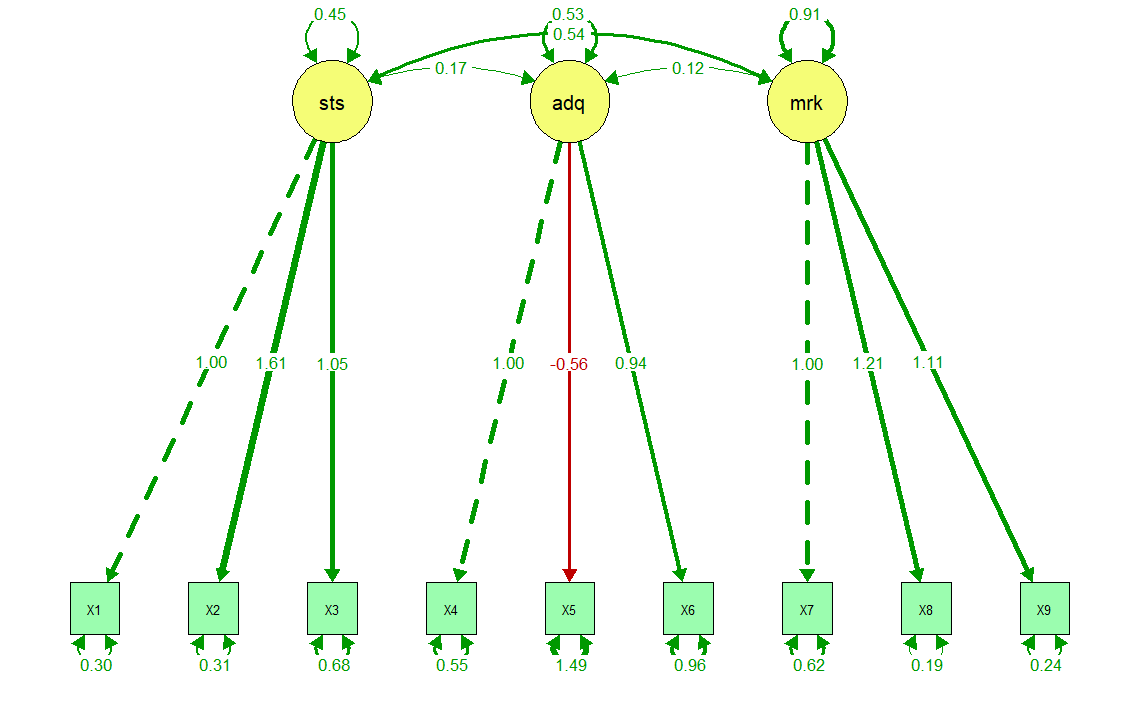
\includegraphics[width=15cm,height=8.5cm]{Imagens/RplotFinal.png}
    \caption{Grafo de correlação das variáveis. Fonte: autores}
    \label{fig:RplotFinal}
\end{figure}

\subsubsection{Análise descritiva}

Para a análise descritiva, os alunos foram divididos em dois grupos, de acordo com dados de triagem (considerados individualmente). No Grupo 1, encontram-se os alunos que: i) trabalham na área há 2 anos ou menos; ii) estão cursando o quarto período ou período menor; iii) têm 24 anos de idade ou menos. No Grupo 2, encontram-se os alunos que: i) trabalham na área há mais de 2 anos; ii) estão cursando o quinto período ou período maior; iii) têm mais de 24 anos de idade. A Tabela 4 mostra de forma numérica como a divisão dos alunos foi feita.

\begin{table}[!ht]
\centering
\begin{tabular}{|c|l|l|l|l|}
\hline
                                                                    & \multicolumn{1}{c|}{\begin{tabular}[c]{@{}c@{}}Condição\\ Grupo 1 (GP1)\end{tabular}} & \multicolumn{1}{c|}{\begin{tabular}[c]{@{}c@{}}Condição\\ Grupo 2 (GP2)\end{tabular}} & \multicolumn{1}{c|}{\begin{tabular}[c]{@{}c@{}}Contagem\\ Grupo 1\end{tabular}} & \multicolumn{1}{c|}{\begin{tabular}[c]{@{}c@{}}Contagem\\ Grupo 2\end{tabular}} \\ \hline
\begin{tabular}[c]{@{}c@{}}Tempo de trabalho\\ na área\end{tabular} & \textless{}= 2 anos                                                                   & \textgreater 2 anos                                                                   & 40                                                                              & 28                                                                              \\ \hline
Período no curso                                                    & \textless{}= 4º periodo                                                               & \textgreater 4º periodo                                                               & 12                                                                              & 56                                                                              \\ \hline
Idade                                                               & \textless{}= 24 anos                                                                  & \textgreater 24 anos                                                                  & 51                                                                              & 17                                                                              \\ \hline
\end{tabular}
\caption{Contagem de integrantes nos grupos. Fonte: autores}
\end{table}

A Tabela 5 exibe uma análise das médias das avaliações das variáveis latentes S e M para cada um dos grupos. A variável A foi desconsiderada, uma vez que não carregou fator e não apresentou valores consideráveis para a confiabilidade composta e o Alfa de Cronbach. Segundo esta análise, é possível verificar que os alunos do Grupo 1 -- menos experientes em termos de tempo de atuação na área e período da graduação e menos maduros em termos de idade -- identificaram maior relação entre as práticas realizadas e o mercado de trabalho e ficaram mais satisfeitos com sua participação nelas do que os alunos do Grupo 2, no geral.

Essa análise descritiva baseada em diferença de médias pode ser considerada estatisticamente válida, pois o cálculo até a mesma considera que o p-valor das variáveis S e M foi aceito mediante os resultados apresentados na Seção 5.3.1.

\begin{table}[!ht]
\centering
\begin{tabular}{|l|l|l|l|}
\hline
\multicolumn{1}{|c|}{\begin{tabular}[c]{@{}c@{}}Média S\\ GP1\end{tabular}} & \multicolumn{1}{c|}{\begin{tabular}[c]{@{}c@{}}Média M\\ GP1\end{tabular}} & \multicolumn{1}{c|}{\begin{tabular}[c]{@{}c@{}}Média S\\ GP2\end{tabular}} & \multicolumn{1}{c|}{\begin{tabular}[c]{@{}c@{}}Média M\\ GP2\end{tabular}} \\ \hline
4,1                                                                         & 3,9                                                                        & 3,7                                                                        & 2,9                                                                        \\ \hline
4                                                                           & 3,8                                                                        & 3,6                                                                        & 2,8                                                                        \\ \hline
4                                                                           & 3,3                                                                        & 3,6                                                                        & 4,2                                                                        \\ \hline
\end{tabular}
\caption{Média obtida por cada grupo nas variáveis latentes. Fonte: autores}
\end{table}

\section{Conclusão e considerações finais}

Como conclusão, tem-se que o ensino orientado a aulas práticas apresentou resultados satisfatórios. Vários alunos demonstraram grande interesse na pesquisa, nas atividades apresentadas e na possível melhoria do ensino orientado pelos princípios \textit{Lean}. Também comentaram que conseguiram perceber a relação das atividades propostas com o mercado de trabalho de \textit{software} e elas podem servir, em certo nível, como base introdutória para técnicas e práticas utilizadas no mercado.

De acordo com a análise de resultados, é possível concluir, em relação aos objetivos deste trabalho, que: i) alunos e professores ficaram satisfeitos com a abordagem -- mesmo que reduzida à etapa Medir -- que foi feita do \textit{Lean Learning}; ii) a proximidade das práticas ao mercado de trabalho de \textit{software} atendeu às expectativas. Entretanto, a adequação das práticas poderia ter sido melhor trabalhada. Houveram queixas em relação ao tempo disponibilizado e divergência em relação a complexidade das práticas, visto que as mesmas foram aplicadas em diversos períodos do curso. A metodologia parece aplicável e viável no contexto das disciplinas estudadas.

Também é possível concluir que um dos caminhos para, pelo menos, iniciar a implementação da abordagem do \textit{Lean Learning} poderia se dar a partir da etapa Medir. Os professores que decidissem adotá-la, poderiam começar utilizando suas próprias práticas, aplicando-as e medindo-as por meio de questionários ou outras ferramentas de coleta de dados, de forma a buscar compreender como elas podem ser continuamente melhoradas, a partir de \textit{feedbacks} constantes dos alunos. Com esses dados em mãos, os professores poderiam implementar, aos poucos e de maneira cíclica, as demais etapas ilustradas na Figura 1, até o processo começar a rodar naturalmente. 

Uma limitação que requer atenção ao avaliar a viabilidade da implementação da abordagem em uma disciplina é o estudo da proximidade existente entre as duas -- neste trabalho, foram selecionadas para estudo somente disciplinas que tinham alguma relação com \textit{Lean Management} ou com áreas mais técnicas do mercado de trabalho de \textit{software}. Também é possível que existam disciplinas que não se encaixem com o modelo proposto, visto que o espaço amostral desta pesquisa se limitou a apenas cinco disciplinas.

Este trabalho trouxe duas contribuições: uma prática e uma teórica. A prática se exprime nos resultados e conclusões apresentadas sobre a eficácia do uso de práticas no ensino. A teórica se dá pelo modelo implementado pela pesquisa, que pode servir como ferramenta para outros estudos. Trabalhos futuros podem vir a investigar a viabilidade da implementação do \textit{Lean Learning} ao curso de Engenharia de \textit{Software} como um todo, analisando outros critérios e abordagens para disciplinas além dos que foram analisados neste estudo. Também pode-se vir a investigar a aplicação do \textit{Lean Learning} a outros cursos de tecnologia e áreas afins da Engenharia de \textit{Software}, uma vez que é possível que o problema estudado neste trabalho também exista para demais cursos.

\section*{Apêndice}

\textbf{A.\quad Perguntas do questionário fechado aos alunos:}
\begin{enumerate}
    \item Você é um aluno(a) da Engenharia de Software?
    Alternativas: Sim ou não
    
    \item Qual o seu sexo biológico?
    Alternativas: Feminino ou Masculino
    
    \item Qual a sua faixa etária?
    Alternativas: Abaixo de 18 anos; 18 a 24 anos; 25 a 35 anos; 35 a 45 anos; Acima de 45 anos
    
    \item Em que período da graduação você se encontra? 
    Alternativas: 1º a 8º período
    
    \item Há quanto tempo você trabalha na área?
    Alternativas: Não trabalho na área ainda; Até 2 anos na área; 2 a 4 anos na área; 4 a 6 anos na área; Mais de 6 anos na área

    \item Numa escala de 1 a 5, em que 1 representa "Insatisfeito" e 5 representa "Muito satisfeito", como você classifica sua satisfação com o aprendizado proporcionado pela atividade proposta?
    Alternativas: de 1 a 5
    
    \item Numa escala de 1 a 5, em que 1 representa "Aprendi pouco" e 5 representa "Aprendi muito", como você classifica o aprendizado que a atividade proposta foi capaz de oferecer?
    Alternativas: de 1 a 5
    
    \item Numa escala de 1 a 5, em que 1 representa "Pouco interesse" e 5 representa "Muito interesse", como você classifica o seu interesse na atividade proposta?
    Alternativas: de 1 a 5
    
    \item Numa escala de 1 a 5, em que 1 representa "Baixo" e 5 representa "Alto", como você classifica seu nível de cumprimento da atividade proposta?
    Alternativas: de 1 a 5
    
    \item Numa escala de 1 a 5, em que 1 representa "Muito fácil" e 5 representa "Muito difícil", como você classifica o nível de dificuldade enfrentado na realização da atividade proposta?
    Alternativas: de 1 a 5
    
    \item Numa escala de 1 a 5, em que 1 representa "Tempo insuficiente" e 5 representa "Tempo mais que suficiente", como você classifica o tempo disponibilizado para a realização da atividade proposta?
    Alternativas: de 1 a 5
    
    \item Numa escala de 1 a 5, em que 1 representa "Pouco próximo" e 5 representa "Muito próximo", como você classifica a proximidade da atividade proposta em relação às práticas e demandas profissionais do mercado?
    Alternativas: de 1 a 5
    
    \item Numa escala de 1 a 5, em que 1 representa "Não ajudou" e 5 representa "Ajudou muito", o quanto você julga que a atividade proposta ajudou na sua compreensão de problemas reais envolvendo o tema da atividade?
    Alternativas: de 1 a 5
    
    \item Numa escala de 1 a 5, em que 1 representa "Não agregou" e 5 representa "Agregou muito", o quanto você julga que a atividade proposta agregou em sua vida profissional?
    Alternativas: de 1 a 5
\end{enumerate}
\textbf{B.\quad Perguntas do questionário fechado aos professores:}
\begin{enumerate}
    \item Numa escala de 1 a 5, na qual 1 representa ``Não estão engajados" e 5 representa ``Estão muito engajados", como você classifica o engajamento que os alunos apresentaram em relação à atividade prática?
    Alternativas: de 1 a 5
    
    \item Numa escala de 1 a 5, na qual 1 representa ``Baixa" e 5 representa ``Alta",  como você classifica a complexidade envolvida na realização da atividade proposta?
    Alternativas: de 1 a 5
    
    \item Numa escala de 1 a 5, na qual 1 representa ``Insatisfatório" e 5 representa ``Muito satisfatório", como você classifica o desempenho que os alunos apresentaram na atividade proposta?
    Alternativas: de 1 a 5
    
    \item Numa escala de 1 a 5, na qual 1 representa ``Pouca dificuldade" e 5 representa ``Muita dificuldade", qual é a sua percepção do nível de dificuldade que os alunos tiveram para executar a atividade prática?
    Alternativas: de 1 a 5
    
    \item Numa escala de 1 a 5, na qual 1 representa ``Pouca proximidade" e 5 representa ``Muita proximidade", qual é a sua percepção do nível de proximidade existente entre a atividade proposta e as práticas e demandas profissionais do mercado?
    Alternativas: de 1 a 5
\end{enumerate}
\textbf{C.\quad Perguntas do questionário aberto aos alunos:}
\begin{enumerate}
    \item Discuta sua percepção geral sobre a atividade prática proposta (dificuldades, aprendizados, pontos positivos e/ou negativos). Busque se expressar sobre tópicos abordados e não abordados pelo questionário fechado.
    
    \item Você tem considerações que possam contribuir para melhorar a atividade, na sua opinião? Caso tenha, por favor, tente se basear na resposta dada à pergunta anterior para responder a esta pergunta.
\end{enumerate}
\textbf{D.\quad Problemas de programação (prática 2):}
\begin{enumerate}
\item Escreva um programa ou método que receba como entrada um vetor de inteiros e imprima como saída o número que representa a moda (ou seja, o número com maior ocorrência no vetor).

\item Escreva um programa ou método que receba como entrada um número inteiro e  imprima como saída o valor de seu fatorial.

\item Escreva um programa ou método que receba como entrada um número inteiro em base decimal e imprima como saída seu valor em binário.

\item Escreva um programa ou método que receba como entrada um número inteiro N e imprima como saída os N primeiros termos da sequência de Fibonacci.
\end{enumerate}
\textbf{E.\quad Links:}

Questionário fechado dos alunos:
http://bit.ly/Fechado-Alunos

Questionário fechado do professor:
http://bit.ly/Fechado-Professores

Questionário aberto dos alunos:
http://bit.ly/Aberto-Alunos

Problemas de programação:
https://bit.ly/tcc-pratica2

\textbf{F.\quad \textit{Script}:}
\begin{figure}
    \centering
    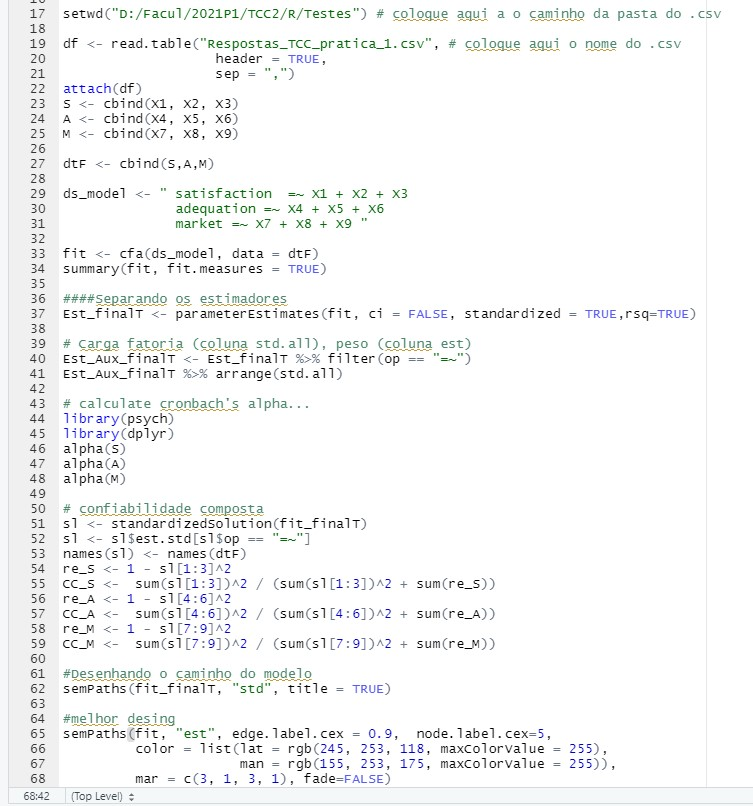
\includegraphics[width=12cm,height=12cm]{Imagens/script.jpg}
    \caption{\textit{script} elaborado em R}
    \label{fig:Processo}
\end{figure}

\ \

\bibliographystyle{sbc}
\bibliography{sbc-template}

\end{document}
